\subsection{Predictive learning via rule ensembles (RuleFit)}
\label{sec:rulefit}

This classifier is a TMVA implementation of Friedman-Popescu's RuleFit\index{RuleFit}
method described in~\cite{RuleFit}. Its idea is to use an 
ensemble\index{Rules!ensemble of} of so-called {\em rules} to create 
a scoring function with good classification power. Each rule $r_i$ is defined by a 
sequence 
of cuts, such as
\begin{align*}
r_1({\bf x}) & = I(x_2<100.0) \cdot I(x_3>35.0)\,,\\
r_2({\bf x}) & = I(0.45<x_4<1.00) \cdot I(x_1>150.0)\,,\\
r_3({\bf x}) & = I(x_3<11.00)\,,
\end{align*}
where the $x_i$ are discriminating input variables, and $I(\dots)$ returns the truth of 
its argument. A rule applied on a given event is non-zero only if all of its cuts are 
satisfied, in which case the rule returns 1.

The easiest way to create an ensemble of rules is to extract it from a forest 
of decision trees (\cf\  Sec.~\ref{sec:bdt}). Every node in a tree (except the root node) 
corresponds to a sequence of cuts required to reach the node from the root node, 
and can be regarded as a rule.  Hence for the tree illustrated in 
Fig.~\ref{fig:decisiontree} on page~\pageref{fig:decisiontree} 
a total of 8 rules can be formed. Linear combinations of the 
rules in the ensemble are created with coefficients (rule weights) calculated using a 
regularised minimisation procedure~\cite{RuleFitMin}. The resulting linear combination 
of all rules defines a {\em score} function (see below) which provides the RuleFit 
response $\yRF({\bf x})$. 

In some cases a very large rule ensemble is required to obtain a competitive 
discrimination between signal and background. A particularly difficult situation 
is when the true (but unknown) scoring function is described by a linear 
combination of the input variables. \index{Rules!linear terms}
In such cases, \eg, a Fisher discriminant
would perform well. To ease the rule optimisation task, a linear combination of the 
input variables is added to the model. The minimisation procedure will then select the 
appropriate coefficients for the rules {\em and} the linear terms. More details are given in 
Sec.~\ref{sec:RuleFitDescript} below.

\subsubsection{Booking options}

The RuleFit classifier is booked via the command:
\begin{codeexample}
\begin{tmvacode}
factory->BookMethod( Types::kRuleFit, "RuleFit", "<options>" );
\end{tmvacode}
\caption[.]{\codeexampleCaptionSize Booking of RuleFit: the first argument is a
            predefined enumerator, the second argument is a 
            user-defined string identifier, and the third argument is the 
            configuration options string. Individual options are separated by a ':'. 
            See Sec.~\ref{sec:usingtmva:booking} for more information on the booking.}
\end{codeexample}
The RuleFit configuration options are given in Option 
Table~\ref{opt:mva::rulefit}.

% ======= input option table ==========================================
\begin{option}[!t]
\input optiontables/MVA__RuleFit.tex
\caption[.]{\optionCaptionSize 
     Configuration options reference for MVA method: {\em RuleFit}.
     Values given are defaults. If predefined categories exist, the default category 
     is marked by a '$\star$'. The options in Option Table~\ref{opt:mva::methodbase} on 
     page~\pageref{opt:mva::methodbase} can also be configured.     
}
\label{opt:mva::rulefit}
\end{option}
% =====================================================================

\subsubsection{Description and implementation}
\label{sec:RuleFitDescript}

As for all TMVA classifiers, the goal of the rule learning is to find a classification 
function $\yRF({\bf x})$ that optimally classifies an event according to the tuple of 
input observations (variables) ${\bf x}$. The classification function is written as
\beq
\label{eq:F}
 \yRF({\bf x}) = a_0 + \sum_{m=1}^{M_R} a_m f_m({\bf x})\,,
\eeq
where the set $\{f_m({\bf x})\}_{M_R}$ forms an ensemble of {\em base learners}
\index{Rules!base learners}
with $M_R$ elements. A base learner may be any discriminating function derived from 
the training data. In our case, they consist of rules and linear terms as described 
in the introduction. The complete model then reads\index{Rules!linear terms}
\beq
\label{eq:FL}
 \yRF({\bf x}) = a_0 + \sum_{m=1}^{M_R} a_m r_m({\bf x}) + \sum_{i=1}^\Nvar b_i x_i\,.
\eeq
To protect against outliers, the variables in the linear terms are modified to
\beq
 x^\prime_i = \min(\delta^{+}_{i},\max(\delta^{-}_{i}))\,,
\eeq
where $\delta^{\pm}_i$ are the lower and upper $\beta$ quantiles\footnote
{
   Quantiles are points taken at regular intervals from the PDF of a random 
   variable. For example, the 0.5 quantile corresponds to the median of the PDF. 
}
of the variable $x_i$. The value of $\beta$ is set by the option \code{LinQuantile}.
If the variables are used ``as is'', they may have an unequal {\em a priori} 
influence relative to the rules. To counter this effect, the variables are normalised
\beq
 x^\prime_i \rightarrow \sigma_{r} \cdot x^\prime_i/\sigma_{i}\,,
\eeq
where $\sigma_{r}$ and $\sigma_{i}$ are the estimated standard deviations 
of an ensemble of rules and the variable $x^\prime_i$, respectively.

\subsubsection*{Rule generation}

The rules are extracted from a forest of\index{Rules!generation of}
decision trees. There are several ways to generate a forest. In the 
current RuleFit implementation, each tree is generated using 
a fraction of the training sample. The fraction depends on which method is
used for generating the forest. Currently two methods are supported (selected
by option \code{ForestType}); \textit{AdaBoost}
and \textit{Random Forest}. The first method is described in Sec.~\ref{sec:bdt_descr}. 
In that case, the whole training set is used for all trees. The diversity is 
obtained through using different event weights for each tree. For a random forest, 
though, the diversity is created by training each tree using random sub-samples. 
If this method is chosen, the fraction is calculated from the training sample size 
$N$ (signal and background) using the empirical formula~\cite{RuleFitWeb}
\beq
\label{eq:sampfrac}
   f =  \min( 0.5, (100.0 +6.0\cdot\sqrt{N})/N)\,.
\eeq
By default, \code{AdaBoost} is used for creation of the forest.
In general it seems to perform better than the random forest.

The topology of each tree is controlled by the
parameters \code{fEventsMin} and \code{fEventsMax}.
They define a range of fractions which are
used to calculate the minimum number of events required in a node for
further splitting. For each tree, a fraction is drawn from a uniform
distribution within the given range. The obtained fraction is then
multiplied with the number of training events used for the tree,
giving the minimum number of events in a node to allow for splitting.
In this way both large trees (small fraction) giving complex rules and
small trees (large fraction) for simple rules are created.  For a
given forest of $N_t$ trees, where each tree has $n_\ell$ leaf nodes,
the maximum number of possible rules is
\beq
   M_{R,\rm max} = \sum_{i=1}^{N_t} 2(n_{\ell,i} - 1)\,.
\eeq
To prune similar rules, a {\em distance} is defined between two
{\em topologically equal} rules. Two rules are topologically equal if 
their cut sequences follow the same variables only differing in their cut values.
The rule distance used in TMVA is then defined by\index{Rules!distance between}
\beq
   \delta_R^2 = \sum_{i} \frac{\delta_{i,L}^2 + \delta_{i,U}^2}{\sigma_i^2}\,,
\label{eq:ruleDist}
\eeq
where $\delta_{i,L(U)}$ is the difference in lower (upper) limit between
the two cuts containing the variable $x_i$, $i=1,\dots,\Nvar$. The difference is 
normalised to the RMS-squared $\sigma_i^2$ of the variable.  Similar rules with 
a distance smaller than \code{RuleMinDist} are removed from the rule
ensemble. The parameter can be tuned to improve speed and to suppress
noise. In principle, this should be achieved in the fitting procedure. However,
pruning the rule ensemble using a distance cut will reduce the fitting time and 
will probably also reduce the number of rules in the final model.
Note that the cut should be used with care since a too large
cut value will deplete the rule ensemble and weaken its classification
performance.

\subsubsection*{Fitting}
\label{sec:rulefitting}

Once the rules are defined, the coefficients in Eq.~(\ref{eq:FL}) are fitted using
\index{Rules!fitting of}
the training data. For details, the fitting method is described in~\cite{RuleFitMin}. 
A brief description is provided below to motivate the corresponding RuleFit options.

A {\em loss function} $L(\yRF({\bf x})|\hat y)$, given by the ``squared-error 
ramp''~\cite{RuleFitMin} 
\beq
   L(\yRF|\hat y) = \left( \hat y - H(\yRF) \right)^2\,,
\eeq
where $H(y) = \max(-1,\min(\yRF,1))$, quantifies the ``cost'' of misclassifying
\index{Rules!loss function of} an event of given true class $\hat y$. The {\em risk} 
$R$ is defined by the expectation value of $L$ with respect to ${\bf x}$ and 
the true class. Since the true distributions are generally not known, the average 
of $N$ training events is used as an estimate\index{Rules!risk of}
\beq
   R = \frac{1}{N}\sum_{i=1}^{N} L(\yRF({\bf x}_i)|\hat y_i)\,.
\label{eq:risk}
\eeq
A line element in the parameter space of the rule weights (given by the vector ${\bf a}$ 
of all coefficients) is then defined by
\index{Rules!fit path}
\beq
\label{eq:rulefitpath}
{\bf a}(\epsilon + \delta \epsilon) = {\bf a}(\epsilon) + \delta \epsilon \cdot {\bf g}(\epsilon)\,,
\eeq
where $\delta \epsilon$ is a positive small increment and ${\bf
  g}(\epsilon)$ is the negative derivative of the estimated risk $R$,
evaluated at ${\bf a}(\epsilon)$.  The estimated risk-gradient is evaluated
using a sub-sample (\code{GDPathEveFrac}) of the training events.

Starting with all weights set to zero, the consecutive application of 
Eq.~(\ref{eq:rulefitpath}) creates a path in the ${\bf a}$ space.
At each step, the procedure selects only the gradients $g_k$
with absolute values greater than a certain fraction ($\tau$) of the largest
gradient. The fraction $\tau$ is an {\em a priori} unknown quantity between 0 and 1.
With $\tau=0$ all gradients will be used at each step, while
only the strongest gradient is selected for $\tau=1$.
A measure of the ``error'' at each step is calculated by evaluating the risk 
(Eq.~\ref{eq:risk}) using the validation sub-sample (\code{GDValidEveFrac}). 
By construction, the risk will always decrease at each step. However, for the 
validation sample the value will increase once the model starts to be overtrained.
Currently, the fitting is crudely stopped when the error measure is larger than 
\code{GDErrScale} times the minimum error found.
The number of steps is controlled by \code{GDNSteps} and the step size ($\delta \epsilon$ in Eq.~\ref{eq:rulefitpath}) by \code{GDStep}.

If the selected $\tau$ (\code{GDTau}) is a negative number, the best value is 
estimated by means of a scan. In such a case several paths are fitted in parallel, 
each with a different value of $\tau$. The number of paths created depend on the 
required precision on $\tau$ given by \code{GDTauPrec}. By only selecting the 
paths being ``close enough'' to the minimum at each step, the speed for 
the scan is kept down.
The path leading to the lowest estimated error is then selected.
Once the best $\tau$ is found, the fitting proceeds until a minimum is found.
A simple example with a few scan points is illustrated 
in Fig.~\ref{fig:rulefitpath}.
\begin{figure}[t]
  \begin{center}
          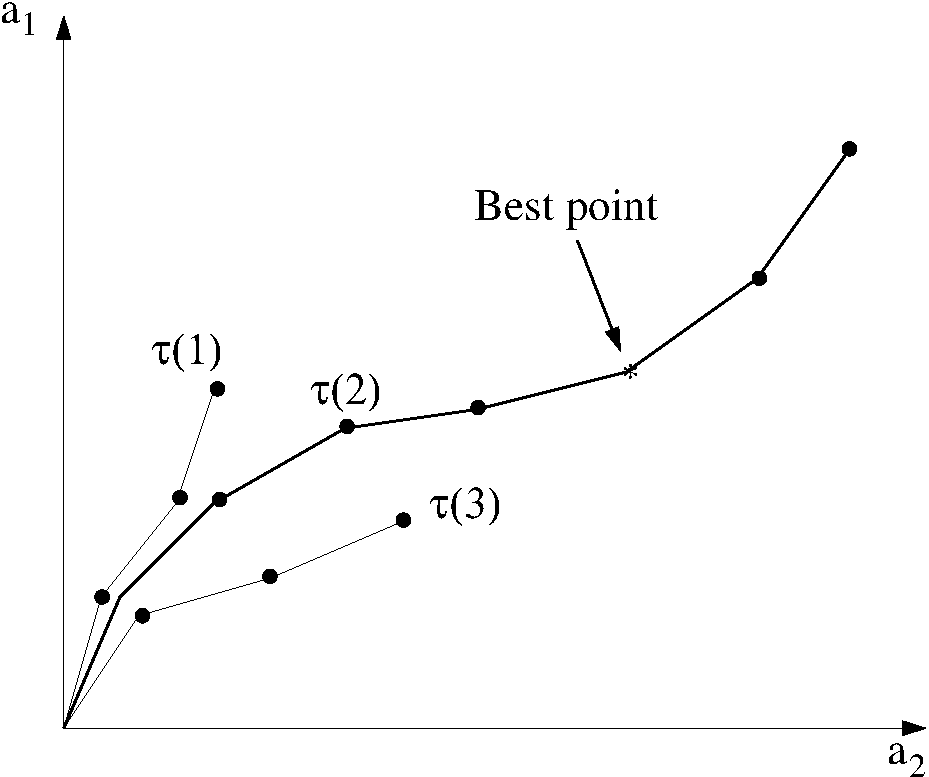
\includegraphics[width=0.55\textwidth]{plots/rulefitpath}
  \end{center}
  \vspace{-0.3cm}
  \caption[.]{An example of a path scan in two dimensions. Each point represents 
              an $\epsilon$ in Eq.~(\ref{eq:rulefitpath}) and each step is given by 
              $\delta\epsilon$. The direction along the path at each point is given 
              by the vector ${\bf g}$. For the first few points, the paths $\tau(1,2,3)$ 
              are created with different values of $\tau$. After a given number of 
              steps, the best path is chosen and the search is continued. It stops 
              when the best point is found. That is, when the estimated error-rate 
              is minimum.}
\label{fig:rulefitpath}
\end{figure}

\subsubsection{Variable ranking}

Since the input variables are normalised, the ranking of variables follows naturally 
from the coefficients of the model. To each rule $m$ ($m=1,\dots,M_R$) can be assigned 
an importance defined by
\beq
\label{eq:rulefit:importance}
 I_m = |a_m| \sqrt{s_m (1.0-s_m)}\,,
\eeq
where $s_m$ is the {\em support} of the rule with the following definition
\beq
 s_m = \frac{1}{N} \sum_{n=1}^N r_m( {\bf x}_n )\,.
\eeq
The support is thus the average response for a given rule on the data sample.
A large support implies that many events pass the cuts of the rule. Hence, such 
rules cannot have strong discriminating power. On the other hand, rules with small 
support only accept few events. They may be important for these few events they accept, 
but they are not in the overall picture. The definition~(\ref{eq:rulefit:importance}) 
for the rule importance suppresses rules with both large and small support.

For the linear terms, the definition of importance is
\beq
 I_i = |b_i|\cdot \sigma_{i}\,,
\eeq
so that variables with small overall variation will be assigned a 
small importance.\index{Rules!variable importance}

A measure of the variable importance may then be defined by
\beq
 J_i = I_i + \sum_{m|x_i\in r_m} I_m/q_m\,,
\eeq
where the sum is over all rules containing the variable $x_i$, and $q_m$ is the number of 
variables used in the rule $r_m$. This is introduced in order to share the importance 
equally between all variables in rules with more than one variable.

\subsubsection{Friedman's module}
\label{sec:friedman}
By setting \code{RuleFitModule} to \code{RFFriedman}, the interface to Friedman's RuleFit 
is selected. To use this module, a separate setup is required. If the module is selected 
in a run prior to setting up the environment, TMVA will stop and give instructions on how 
to proceed. A command sequence to setup Friedman's RuleFit in a UNIX environment is:
\begin{codeexample}
\begin{tmvacode}
~> mkdir rulefit
~> cd rulefit
~> wget http://www-stat.stanford.edu/~jhf/r-rulefit/linux/rf_go.exe
~> chmod +x rf_go.exe
\end{tmvacode}
\caption[.]{\codeexampleCaptionSize The first line creates a working directory 
            for Friedman's module. In the third line, the binary executable is fetched 
            from the official web-site. Finally, it is made sure that the module
            is executable.}
\end{codeexample}
As of this writing, binaries exists only for Linux and Windows. Check J.~Friedman's 
home page at \url{http://www-stat.stanford.edu/~jhf} for updated information.
When running this module from TMVA, make sure that the option \code{RFWorkDir}
is set to the proper working directory (default is \code{./rulefit}).
Also note that only the following options are used:
\code{Model}, \code{RFWorkDir}, \code{RFNrules}, \code{RFNendnodes}, 
\code{GDNSteps}, \code{GDStep} and \code{GDErrScale}. The options \code{RFNrules} and \code{RFNendnodes} correspond in the package by Friedman-Popescu to the options \code{max.rules} and \code{tree.size}, respectively. For more details, the reader is referred to Friedman's RuleFit manual~\cite{RuleFitWeb}. 

\subsubsection*{Technical note}
The module \code{rf_go.exe} communicates with the user by means of both ASCII and 
binary files. This makes the input/output from the module machine dependant. TMVA 
reads the output from \code{rf_go.exe} and produces the normal machine independent 
weight (or class) file. This can then be used in other applications and environments.

\subsubsection{Performance}

Rule ensemble based learning machines are not yet well known within the
HEP community, although they start to receive some
attention~\cite{RuleSusy}. Apart from RuleFit~\cite{RuleFit}
other rule ensemble learners exists, such as SLIPPER~\cite{SLIPPER}.

The TMVA implementation of RuleFit follows closely the original design
described in Ref.~\cite{RuleFit}. Currently the performance is however slightly
less robust than the one of the Friedman-Popescu package. Also, the experience 
using the method is still scarce at the time of this writing.

To optimise the performance of RuleFit several
strategies can be employed.  The training consists of two steps, rule
generation and rule ensemble fitting. One approach is to modify the
complexity of the generated rule ensemble by changing either the
number of trees in the forest, or the complexity of each tree. In general, 
large tree ensembles with varying trees sizes perform better than short non-complex
ones. The drawback is of course that fitting becomes slow.  However, if the
fitting performs well, it is likely that a large amount of rules will
have small or zero coefficients. These can be removed, thus
simplifying the ensemble. The fitting performance can be improved by 
increasing the number of steps along with using a smaller step size. Again, 
this will be at the cost of speed performance although only at the training stage.
The setting for the parameter $\tau$ may greatly affect the result. Currently 
an automatic scan is performed by default. In general, it should find the 
optimum $\tau$. If in doubt , the user may set the value explicitly.
In any case, the user is initially advised to use the automatic scan option to 
derive the best path.
